% ------------------------------------------------------------------------------------------------------------------------------------------------
\chapter{Cluster scaling and performance analysis}
\label{chap:perf-scalability}

This section will focus on analysing as well as presenting improvements to the cluster deployment which can and have been applied to the Hadoop cluster leveraged by the Analyser application presented in previous chapters.

Section \ref{sec:scaling-hadoop} describes the multitude of challanges and problems encountered while scaling Hadoop cluster. It also describes three of the applied scaling and optimisation methods in detail -- including configuration changes as well as adding more nodes to the cluster.

Section \ref{sec:optimising-hbase} discusses HBase specific optimisations that can be performed during application and data representation design. While all optimisations described in the previous section, which touch Hadoop's infrastructure also directly impact HBase performance, some very specific topics -- such as utilising HBase's guarantees about it's globally sorted row key and guaranteed random access times to specific row-keys make this topic worthy if it's own section.

Section \ref{sec:scaling-akka} will briefly explain scalability concerns related to an Akka based cluster deployment, yet as this component has not been as critical to overal system performance as the Analyser and Hadoop cluster, the Akka cluster has been deemed ''good enough'' for the scope of this paper.

Lastly Section \ref{sec:scaling-summary} will summarise the findings from the scaling experiments conducted in the previous sections, by stating general recommendations and hints for scaling systems that process larget amounts of data.

% ------------------------------------------------------------------------------------------------------------------------------------------------
\section{Scaling the Analyser's Hadoop Cluster}
\label{sec:scaling-hadoop}
This section will focus on analysing and tuning the various settings of the Hadoop cluster deployed for the previously described Analyser application. Subsections focus on tuning the cluster on a setting--by--setting basis yet the tuning will always be enforced by a business need, which in this case will be represented as the need to speed up processing of the map reduce pipelines producing results which were explained in Chapter \ref{chap:analysis-examples}.

\subsection{Storing images on HDFS, while avoiding the ''Small Files Problem''}
\label{sec:sequence-files}
Most algorithms used in Oculus operate on a frame-by-frame basis, which means that it is most natural to store all data as ''data for frame 343 from movie XYZ''. This applies to everything from plain bitmap data of a frame to metrics such as histograms of colours of a given frame or other metadata like the extracted text content found in this frame.

Sadly this abstraction does \textit{not} work nicely with Hadoop, it would cause the well--known ''small-files problem'' which leads to \textit{major} performance degradation of the Hadoop cluster is left unadressed. This section will focus on explaining the problem and what steps have been taken to prevent it from manifesting in the presence of millions of ''frame-by-frame'' pieces of data.

Hadoop uses so called ''blocks'' as smallest atomic unit that can be used to move data between the cluster.
The default block size is set to \textit{64 megabytes} on most Hadoop distributions.

This also means that if the DFS takes a write of one file (assuming the \textit{replication factor} equals 1) it will use up one block. By itself this is not worrying, because other than in traditional (local) file systems such as EXT3 for example, when we store N bytes in a block on HDFS,
the the file system can still use block's unused space. Figure \ref{fig:no-sequence-file} shows the structure of a block storing only one frame of a movie.

\begin{figure}[ch!]
  \centering
  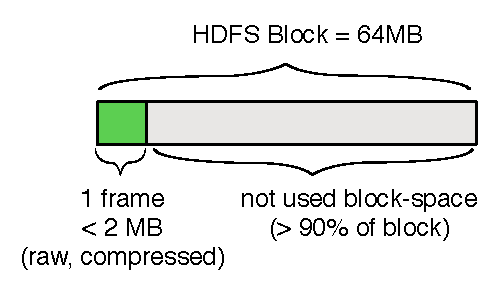
\includegraphics[scale=0.9]{diagrams/no-sequence-file.pdf}
  \caption{When storing a small file in HDFS, it still takes up an entire block. The grey space is not wasted on disk, but causes \textit{name-node} to store 1 block entry in memory.}
  \label{fig:no-sequence-file}
\end{figure}

The problem stemming from writing small files manifests not directly by impacting the used disk space, but in increasing memory usage in the clusters so called \textit{name-node}. The name-node is responsible for acting as a lookup table for locating the blocks in the cluster. Since name-node has to keep 150KB of metadata for each block in the cluster, creating more blocks than we actually need quickly forces the name-node to use so much memory, that it may run into long garbage collection pauses, degrading the entire cluster's performance. To put precise numbers to this -- if we would be able to store 500MB of data in an optimal way, storing them on HDFS would use 8 blocks -- causing the name node to use approximately 1KB of metadata. On the other hand, storing this data in chunks of 2MB (for example by storing each frame of a movie, uncompressed) would use up 250 HDFS blocks, which results in additional 36KB of memory used on the name-node, which is 4.5 times as much (28KB more) as with optimally storing the data! Since we are talking about hundreds of thousands of files, such waste causes a tremendous unneeded load on the name-node.

It should be also noted, that when running map-reduce jobs, Hadoop will by default start one map task for each block it's processing in the given Job. Spinning up a task is an expensive process, so this too is a cause for performance degradation, since having small files causes more \textit{Map tasks} being issued for the same amount of actual data Hadoop will spend more time waiting for tasks to finish starting and collecting data from them than it would have to.

% ------------------------------------------------------------------------------------------------------------------------------------------------
\subsubsection{Sequence Files}
\label{sequence-file}
The solution applied in the implemented system to resolve the small files problem is based on a technique called ''Sequence Files'', which are a manually controlled layer of abstraction on top of HDFS blocks. There are multiple Sequence file formats accepted by the common utilities that Hadoop provides \cite{hadoop-seq-files} but they all are \textit{binary header-prefixed key-value formats}, as visualised Figure \ref{fig:sequence-file}.


\begin{figure}[ch!]
  \centering
  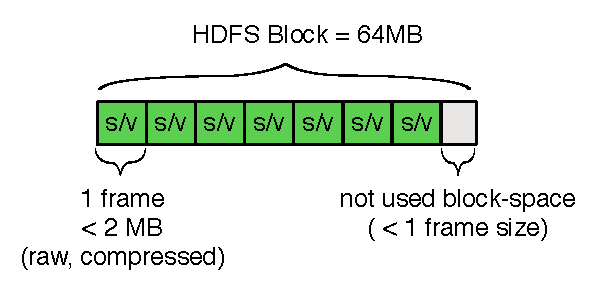
\includegraphics[scale=0.9]{diagrams/sequence-file.pdf}
  \caption{A SequenceFile allows storing of multiple small chunks of data in one HDFS Block.}
  \label{fig:sequence-file}
\end{figure}

Using Sequence Files resolves all previously described problems related to small files on top of HDFS. Files are no longer ''small'', at least in Hadoop's perception,
since access of frames of a movie is most often bound to access other frames of this movie we don't suffer any drawbacks from such storage format.

Another solution that could have been applied here is the use of HBase and it's key-value design instead of the explicit use of Sequence Files, yet this would not yield much performance nor storage benefits as HBase stores it's Table data in a very similar format as Sequence Files. The one benefit from using HBase in order to avoid the small files problem would have been random access to any frame, not to ''frames of this movie'', but since I don't have such access patterns and it would complicate the design of the system I decided to use Sequence Files instead.



% ------------------------------------------------------------------------------------------------------------------------------------------------
\subsection{Tuning replication factors, for increased job computation speed}
\label{sec:tuning-replication-factors}
One of the many tuneable aspects of Hadoop deployments that can have a very high impact on the clusters performance is the \textit{replication factor}, which stands for ''the number of datanodes a piece of data is replicated to''. This section will explain in detail how a tuning this factor, and leveraging Hadoop's scheduling mechanisms can be tweaked to trade of storage space (higher replication factors) to faster execution times of jobs.

Hadoop's primary strength in big data applications lies within leveraging \textit{data locallity} whenever possible. The concept of data locallity means that instead of moving the data around in the cluster, to a node where the application is running, the Task Scheduler will try find such ''map slots'' (multiple such slots can be assigned to one data node) that the data the job needs to process will be local to the node the slot resides on. Effectively this means that application code (jar and class files) will be sent to the executing server, and not the inverse. The rationale behind this measure is that the amounts of data are way bigger than the size of applications in these kinds of systems -- thus, avoiding to move the data can save both costs and precious time.


\begin{figure}[ch!]
  \centering
  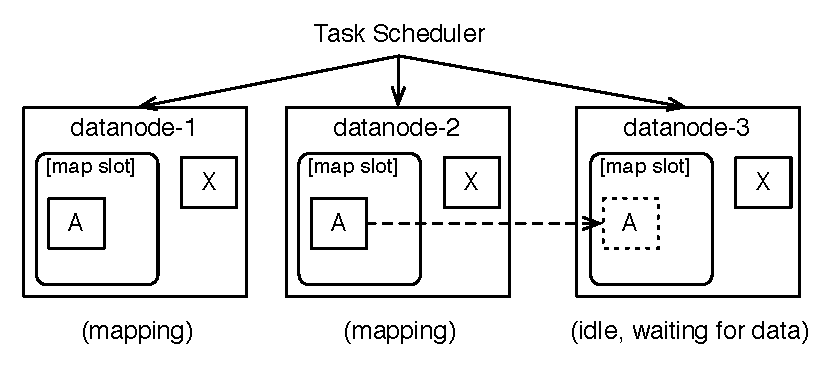
\includegraphics[width=\textwidth]{img/forced-data-replication.pdf}
  \label{fig:replication-ad-hoc}
  \caption{Three node cluster, with idle 3rd node; Scheduler will replicate data A while running the Job, in order to start a task requireing A on the 3rd idle node.}
\end{figure}


While data locallity is a \textit{priority} for the scheduler, it is by no means a hard requirement. In a scenario outlined in Figure \ref{fig:replication-ad-hoc} a job has been submitted to a 3-node cluster. The replication factor in the cluster is set to 2 -- which can be noticed by the number of times each piece of data is replicated among the datanodes. In the absence of any other jobs scheduled on the cluster, the fair--scheduler will decide to use the 3rd data node in order to accelerate the processing of the job, even though it does not have the required piece of data located on it (splits of A). Replicating the data over to datanode-3 is quite costly, and even though it may speed-up the total compute time, we loose time on transfering the data in an ad-hoc fashion.

By tweaking the replication factor for the given file, which we expect to be needed on more nodes, we can speed up the total compute time of a given job. In order to change the replication factor of a given path, one can use either the Java APIs or the hadoop command line tool, as shown in Listing \ref{lst:cli-change-replication}.

\begin{lstlisting}[caption={Explicitly changing the replication factor on a path using command line tools}, label={lst:cli-change-replication}]
hadoop dfs -setrep -R -w 3 /oculus/source/e98uKex3hSw.mp4.seq
\end{lstlisting}

By increasing the replication factor of paths that we know they will be used in many mappers, we can increase the number of data-local slots available to the scheduler, and avoid having to migrate the data in an ad-hoc fashion. Of course, the tradeoff is requireing even more disk space in the cluster, but it is well worth considering to raise the replication factor of a path while it is ''hot'', and lowering it afterwards.

\begin{figure}
  \centering
  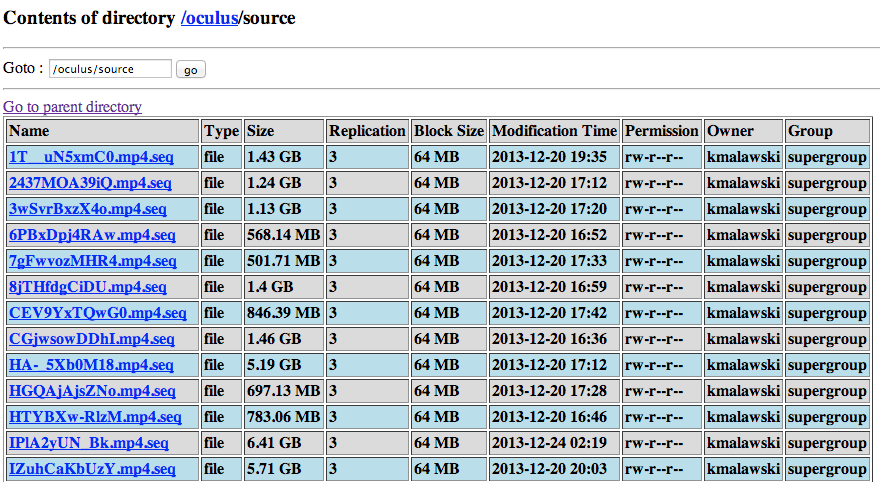
\includegraphics[width=\textwidth]{img/hadoop/hdfs_show-replication}
  \label{fig:hdfs-replication-factors}
  \caption{HDFS on-line browser, running on datanode (port: 50075), displaying replication factors of files (4th column)}
\end{figure}

The replication factor of a file (or path) is such an important value, it's usually always displayed along side any file listing within the Hadoop UIs (see Figure \ref{fig:hdfs-replication-factors}) as well as command line tools. It should also be noted that it is impossible to set the replication factor to a higher number than there are datanodes present in the cluster -- as the replication requirement would not be possible to be fulfilled.


\subsection{Tuning the Cluster's size, in conjunction with replication factors}
\label{sec:tuning-number-of-nodes}
Hadoop aims to deliver on the promise of ''nearly linear horizontal scalability'', which means that speed-up expirienced from adding more nodes to the cluster should impact the processing times positively in a linear fashion. Of course, adding more nodes also means that operational costs are higher, so one has to ballance the number of nodes with their fine-tuning as well as project needs. In order to test the systems behavior, the cluster was configured with 1 map slot on each datanode, and was initially running using 3 datanodes. This section aims to verify the horizontal scalability of the produced cluster, in the case of CPU intensive tasks -- such as computing phashes and histograms from movies (the pre-processing step as explained in Chapter \ref{chap:analysis-examples}.

Because the Map Reduce framework relies on parallelising computing of the map function supplied by the user, the goal of the cluster administrator should be to enable the maximum number of map slots. A map slot is defined as one ''slot'' in which the task scheduler may allocate work, in order to process a part of the map computation. The same can be specified for the reduce step, in which case one refers to \textit{reduce slots}.

\subsubsection{Growing the cluster}
\label{sec:growing-the-cluster}
With the base size of the cluster being 3 nodes (with one virtual machine hosting the namenode as well as a datanode, and the rest hosting only datanodes), this section aims to determine the horizontal scalability of the cluster, by sheer adding of datanodes to the hadoop cluster.

Adding nodes to the cluster is a very simple operation, and can be performed without any disruption of the already running cluster. During the tests performed for this section, additional VMs have been provisioned and added to the cluster by using the commands shown in Listing \ref{lst:adding-new-node-cluster}. It should be noted that the provisioned VMs would re-use an existing snapshot image of an instance prepared using OpsCode Chef, which is an configuration provisioning tool explained in detail in Appendix \ref{app:chef}. 

\textbf{The average time from starting a new node on Google Compute Engine, and it joining the Hadoop cluster is \textit{less than 1 minute} -- including the time to provision the fresh virtual machine!}

\newpage
\begin{lstlisting}[caption={Complete listing of adding a new worker node to the cluster, using GCE}, label={lst:adding-new-node-cluster}]
// provision new instance
gcutil --service_version="v1" --project="oculus-hadoop" adddisk "oculus-4b" --zone="us-central1-a" --source_snapshot="oculus-slave-snapshot"

gcutil --service_version="v1" --project="oculus-hadoop" addinstance "oculus-4b" --zone="us-central1-a" --machine_type="n1-standard-1" --network="default" --external_ip_address="ephemeral" --service_account_scopes="https://www.googleapis.com/auth/..." --tags="hadoop,datanode,hbase" --disk="oculus-4b,deviceName=oculus-4b,mode=READ_WRITE,boot" --auto_delete_boot_disk="true"

// obtain ip address
gcutil getinstance oculus-3b | grep ip
// ip               10.240.80.181
// external-ip  146.148.47.191

// add internal ip to namenode masters config
gcutil ssh oculus-master
echo "10.240.80.181" >> /opt/hadoop.1.2.1/conf/slaves

// start workers on added nodes
/opt/hadoop-1.2.2/start-all.sh

// add node aliases to local hosts
echo "146.148.47.191  oculus-3b" >> /etc/hosts
\end{lstlisting}

The job used to measure the impact of adding new nodes was the most CPU intensive task present in the Oculus workflow, which is: computing the perceptual hash of each frame of a given movie. The movie selected for the process was the previously introduced ''Big Buck Bunny'' movie, amounting a total of 6.38 GB of frame data to process, split among 103 HDFS Blocks (each roughly 64 MB in size). Thanks to this large number of blocks, the task scheduler should be able to efficiently distribute the work to even large numbers of worker nodes. In fact, as visible on Figure \ref{fig:ten-mappers} with 10 mappers (10 datanodes, with 1 map slot each) are executing tasks from the same job in parallel, causing an obvious speedup in Map comptation.


\begin{figure}[ch!]
  \centering
  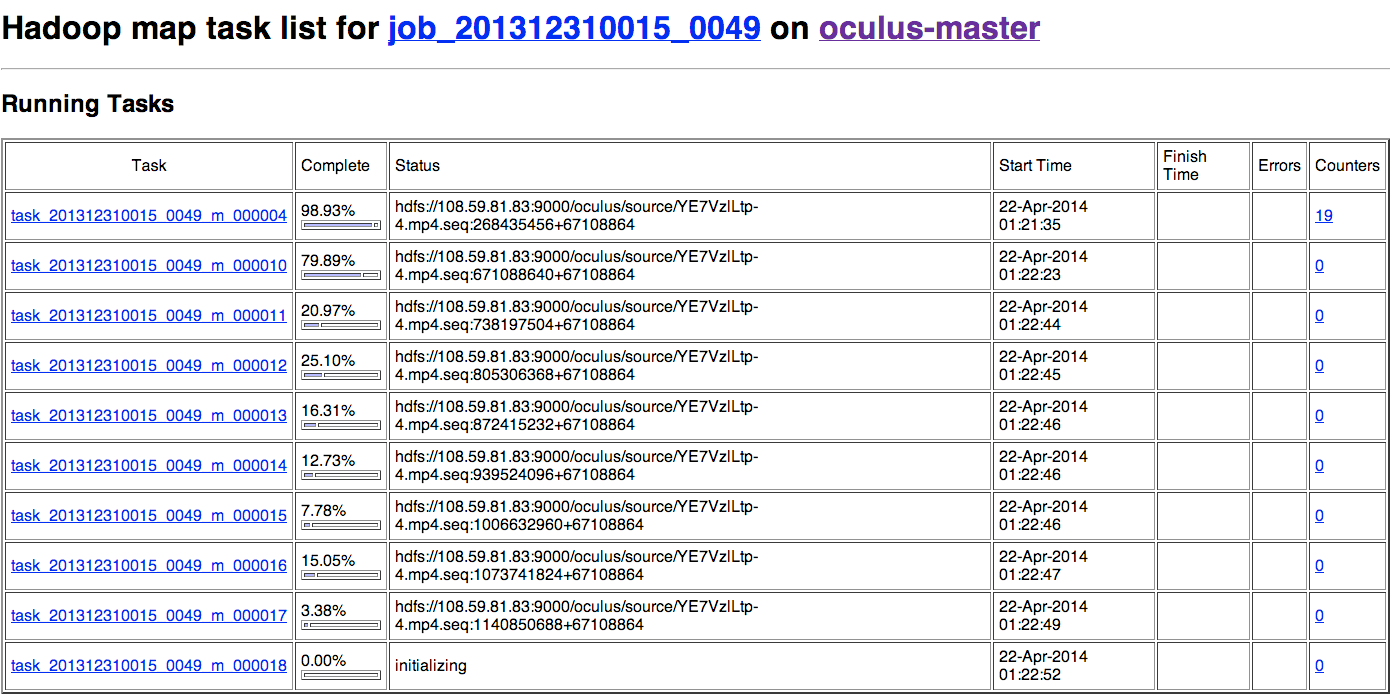
\includegraphics[width=\textwidth]{img/hadoop/10tasks-parallel}
  \label{fig:ten-mappers}
  \caption{Fragment of Web-UI interface displaying the progress of map tasks in the cluster consisting of 10 physical nodes, with one map slot each.}
\end{figure}

Before explaining the results of the performed scalability tests, one more term needs to be introduced. Tasks can be executed in a number of different ways -- that is, they may be executed strictly local to the data they work on, or just ''near the data the task requires'' or really ''far away from the data the task requires'' -- these intuitive definitions have their named counterparts which are measured and reported for every run of a Map Reduce job, namely those types of Tasks are:

\begin{itemize}
  \item \textbf{Data Local Task} -- the Task is executed on the same datanode on which the data it requires resides. No data transfer between nodes is required for the task to start. This is the optimal type of Task, and one should aim at maximising their number during an execution of Map Reduce jobs.
  \item \textbf{Rack Local Task} -- the Task is executed on a datanode that is located on the same rack (in the datacenter) as the node that the data it requires resides. This kind of task will require the data to be transfered between the two hosts, but since they are located on the same rack the transfer cost is still relatively small.
  \item \textbf{Remaining Tasks} -- tasks that are not Data Local do not have a name of their own, and are not reported directly. Instead one aims to maximise the number of Data and Rack Local tasks, with the rest being simply \verb|notLocalTasks = totalTasks - dataLocalTasks - rackLocalTasks|. These tasks require transfering the data across the network for the job to start, and should be avoided at all costs -- in our use-cases it was possible to avoid triggering even one of these tasks.
\end{itemize}

The first row in Table \ref{table:more-nodes-results} represents the theoretical time to execute the job using only one node -- the aproximated time to complete the job using one thread (mapper) was calculated by calculating the average time of computing one split of data, which is equal to: \textit{47 seconds}. Other time characteristics of computing one task are listed, for reference, in Table \ref{table:task-compute-time}.

\begin{table}[hbt]
  \centering
  \begin{tabular}{|c|c|}
  \hline
    \textbf{Characteristic} & \textbf{Value (seconds)} \\ \hline
    min                     & 41     \\ \hline
    max                     & 71     \\ \hline
    avg                 	    & 47.41  \\ \hline
    stddev                  & 4.33   \\ \hline
  \end{tabular}
  \label{table:time-task}
  \caption{Time characteristics of executing one Task of the analysed job.}
\end{table}


The experiment was then expanded to more nodes, and afterwards the replication factor was increased to increase the chance of triggering Data Local tasks. Results of the experiment are listed in Table \ref{table:more-nodes-results}.

\begin{table}[hbt]
  \centering
  \begin{tabular}{|c c|c|c|c|c|c|}
  \hline
    \multicolumn{2}{|c|}{\textbf{Cluster configuration}} & \multicolumn{2}{|c|}{\textbf{Tasks executed}} & \multicolumn{3}{|c|}{\textbf{Performance}} \\ \hline
    Nr of nodes & Replication & Data local & Rack local   & Time              & Speed-up    & Abs. speed-up \\ \hline
    1 node (simulated)    & 1 & 103 & 0                   & aprox. 87 mins    & --          & --            \\ \hline
    3 nodes               & 3 & 103 & 0                   & 27 mins, 14 sec   & 3.19        & 3.19          \\ \hline
    4 nodes               & 3 & 89  & 14                  & 21 mins, 53 sec   & 1.25        & 3.98          \\ \hline
    7 nodes               & 4 & 67  & 36                  & 12 mins, 37 sec   & 1.73        & 6.90          \\ \hline
    10 nodes              & 4 & 54  & 49                  & 9 mins, 1 sec     & 1.40        & 9.65          \\       
                          & 6 & 99  & 4                   & 8 mins, 49 sec    & 1.02 (1.43) & 9.87          \\ \hline
  \end{tabular}
  \caption{Computation speed-up by adding nodes, and increasing replication factors, leading to increased data locality for exacuted jobs.}
  \label{tab:more-nodes-results}
\end{table}

Analysing Table \ref{table:more-nodes-results} yields very interesting results. The most interesting metric in our case if of course the absolute speed-up of the process, yet the relative speed-up (as measured between previous and current configuration) is also quite interesting -- especialy in cases when the replication factor was modified.

The first notable and interesting difference is of course between running the job on 1 node to 3 nodes, with the replication factor equal to the number of nodes to the cluster. This has the obvious effect of all tasks being executed local to the data they require (as each node has all the data). The total speed-up is around 3, which would indicate linear scalability in this case. Yet becuase of still small numerf of nodes, and everything being executed locally, this case is not very interesting from the ''introduction of cluster communication overhear'' perspective.

The next notable effect demonstrated during this experiment is visible when scaling the cluster to 4 nodes, without increasing the replication factor (which stayed at 3). This forced the cluster to execute Rack Local tasks for the first time. The scheduler was forced into scheduling 14 tasks on nodes that did not have the data locally available, although it managed to schedule them on Rack Local tasks -- which still is an acceptable choice for most computations.

After scaling the cluster to 10 nodes, and updating the replication factor to 4 -- specifically chosen because it being ''slightly bellow half the number of the nodes'', one can observe a significant drop in tasks being executed Data Locally -- this is because the scheduler has more nodes available, and since they are idle, it decides to use them instead of keeping them idle -- it will do so, even if there are no Data Local slots available. In the end it still results in an \verb|1.4| speed-up as related to the 7 nodes scenario, even if the number of Rack Local taks has incresed by a factor of \verb|3.5|.

The last, and perhaps most interestning measured change to the cluster involved increasing the replication factor on an 10 nodes cluster to \verb|6| -- so that more than half of the servers would host the same piece of data. After waiting for the data to be propagated (notice that datanodes undergoing heavy migration can appear unavailable to the cluster), the job was started again. This time, even though the relative number of nodes that have the data locally was not so much different (''slightly more thank half of the nodes'') as in the 7 nodes scenario, it's highly interesting to see that \verb|99| out of \verb|103| (96\%) tasks were executed as Data Local tasks. While the change in the numbers of Data Local tasks executed seems fantastic, the difference in relative speed-up between replication factors 4 and 6 in this case in relation to the 7 nodes case was a mere \verb|0.03| precentage points, and around 11 seconds, a speed-up most likely not not worth the added data duplication introduced to the cluster -- which also has a financial backlash (more data duplication, resulting in the need of even more disks, resulting in the need of even more servers).

\begin{figure}[ch!]
  \centering
  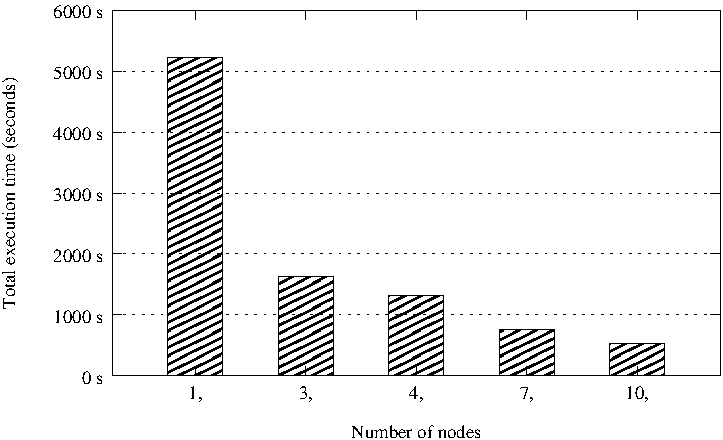
\includegraphics[width=0.80\textwidth]{img/hadoop/nodes-perf.pdf}
  \label{fig:nodes-pers-graph}
  \caption{Fragment of Web-UI interface displaying the progress of map tasks in the cluster consisting of 10 physical nodes, with one map slot each.}
\end{figure}

In order to summarise this section, one last observation should be made about Table \ref{table:more-nodes-results}, namely: in respect of adding more nodes to the Hadoop cluster, it seems that it scales nearly linear, as can be seen by comparing the number of nodes compared to the absolute speed-up, for example -- when running a cluster with \verb|10| nodes, the absolute speedup in relation to running on one node was \verb|9.87 times|, which is very near to a full 10. Thanks to this experiment one can conclude that (at least to such numbers of nodes) Hadoop is in fact \textit{nearly linearili scalable}, which is considered quite an achievement and would serve the growing-over-time needs of a data processing platform very well.


% ------------------------------------------------------------------------------------------
\subsection{Tuning cluster utilization through setting map / reduce slot numbers}
\label{sec:tuning-cluster-utilisation}
The last investigated option available for increasing cluster utilisation investigated was the \verb|mapred.map.tasks| setting and it's corresponding \verb|mapred.reduce.tasks|, as hinted by Eric Sammer in \cite{hadoop-ops}.

\begin{figure}[ch!]
  \centering
  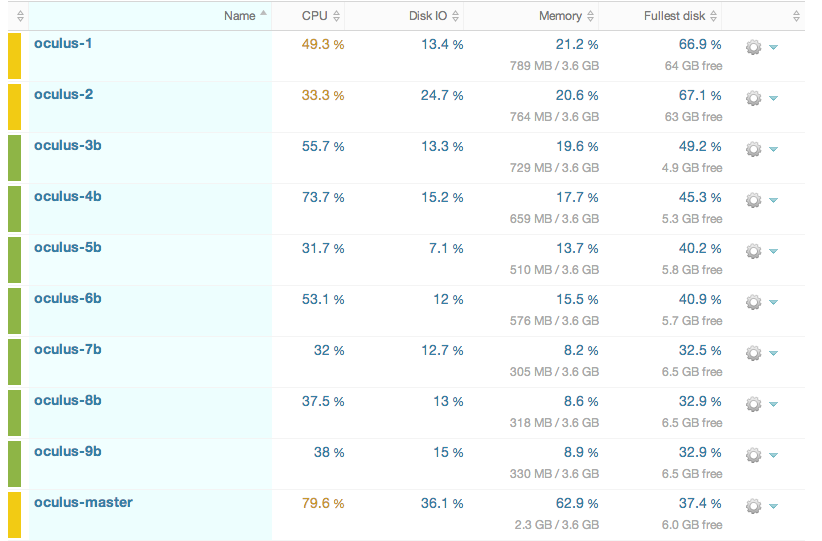
\includegraphics[width=0.8\textwidth]{img/hadoop/10nodes-newrelic-suffering-from-no-data-locallity}
  \label{fig:ten-under-utilised-cluster}
  \caption{An example of an underutilised cluster, where each node has 1 map and 1 reduce slot, yet the computed task is not draining the available CPU time, leading to wasting precious compute time.}
\end{figure}

These settings influence the number of Map and Reduce ''slots'' available for the scheduler on each node. By default these are set to 1 map task for each physical CPU available on the node (as can be seen on Figure \ref{fig:four-nodes-config}, where \textit{oculus-3-cpu} has 2 physical CPUs, and was automatically assigned 2 map and reduce slots). When running multiple example jobs on the cluster, it was discovered that some ''low utilisation'' jobs would needlessly occupy precious map slots on the cluster -- leading to such worst-case scenarios as depicted on Figure \ref{fig:ten-under-utilised-cluster}, where all nodes (all of which are of type: \textit{n1-standard-1 (1 vCPU, 3.8 GB memory)}) are processing one task and which occupies 100\% of their task slots (because each has 1 CPU), yet the task is \textit{not} CPU intensive, which leads to wasting precious CPU time. It would be much more efficient to allow these nodes to run at least 2 map and reduce tasks at the same time - since they they won't be competing for each other's CPU time.

\begin{figure}[ch!]
  \centering
  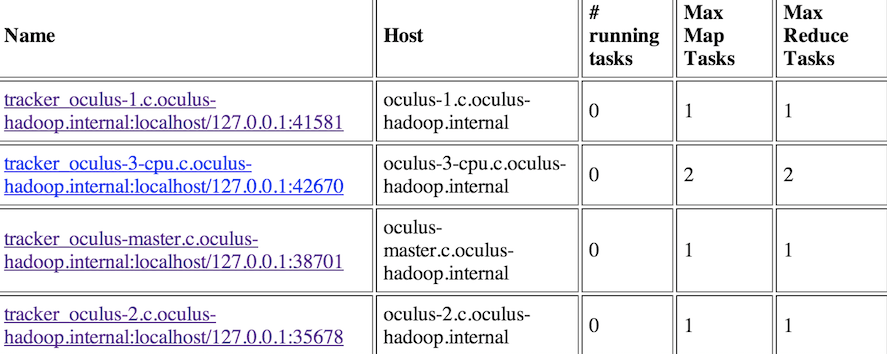
\includegraphics[width=\textwidth]{img/hadoop/4node-cluster-config}
  \label{fig:four-nodes-config}
  \caption{Fragment of Web-UI displaying the connected datanodes. The oculus-3 node is an high-cpu instance, and has more slots than the remaining nodes.}
\end{figure}

In order to avoid cluster under utilisation as seen on Figure \ref{fig:ten-under-utilised-cluster} (where 10 nodes are working, yet the vast majority of them only utilises around 30\% of their CPU), the number of concurrent tasks to be executed on one node was increased to 2 map and 2 reduce tasks. Literature recommends using \verb|rount(1.5 * nrOfCpus)| tasks per node, yet this setting should be always accustomed to the workload a cluster is expiriencing. Having this in mind, a scaled down cluster may actually be more efficient on processing such jobs. The changed configuration included 4 nodes, all of which were set-up fo host 2 map slots and 2 reduce slots. The CPU load on the cluster in such configuration, performing the same job as seen on Figure \ref{fig:four-nodes-config}, can be seen on Figure \ref{fig:cpu-load-during-job}.

\begin{figure}[ch!]
  \centering
  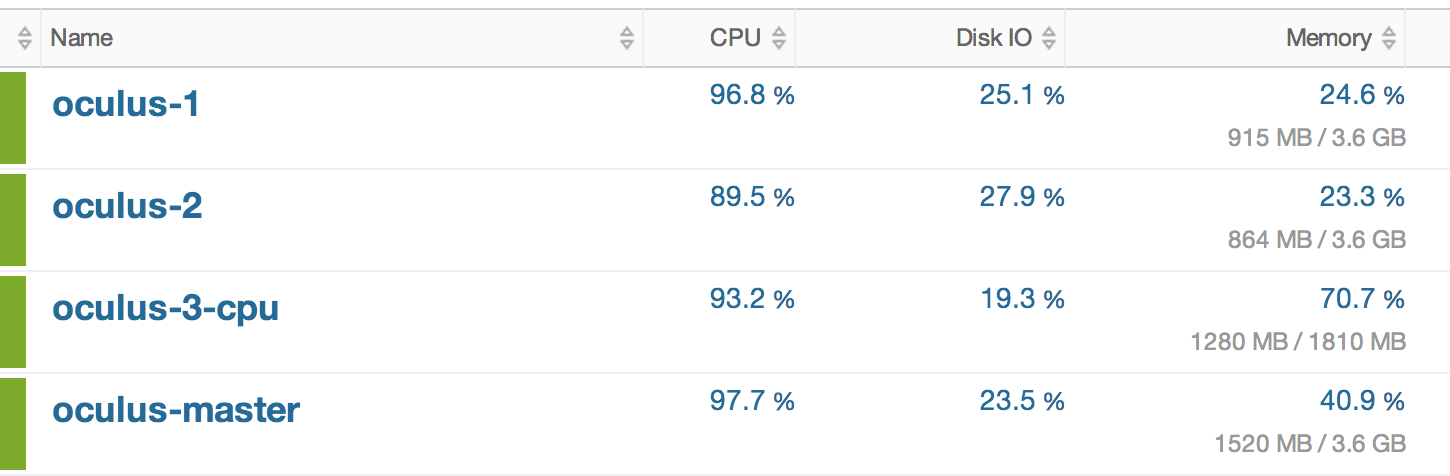
\includegraphics[width=\textwidth]{img/hadoop/monitoring-during-processing}
  \label{fig:cpu-load-during-job}
  \caption{Screenshot of New Relic (cluster monitoring software) displaying CPU and memory utilisation during the execution of an CPU intensive map reduce job.}
\end{figure}

It is worth keeping in mind that cost efficiency usually is also an important business need and simply adding more servers sometimes isn't an available option. Even more so, sometimes we may end up over provisioning servers -- as seen in Figure \ref{fig:ten-under-utilised-cluster}, so while simply adding more servers is very tempting and usually works very well on Hadoop clusters (as seen in Section \ref{sec:tuning-number-of-nodes}), one should always first try to fine tune the cluster to the specific work-load it is experiencing. In the case shown in this section, a fine-tuned 4 node cluster was able to perform almost as good (for this set of jobs), as the under utilised 10 node cluster. In real life clusters will always execute very different workloads at the same time, so it may be very hard to fine tune it for very percise scenarios, yet the effort of changing configurations of cluster members can sometimes prevent the need of adding more servers, so it should be always considered first -- unless a long term cluster expansion (e.g. ''adding 100 nodes, in the next 2 months'') is planned directly.

% ------------------------------------------------------------------------------------------------------------------------------------------------
%\section{Denormalisation as way to increase lookup performance in the Analyser's HBase interactions}
%\label{sec:optimising-hbase}
%
%While all performance optimisations mentioned in the Section about Hadoop scaling, directly impact HBase performance



% ------------------------------------------------------------------------------------------------------------------------------------------------
\section{Scaling out the Loader's Akka Cluster}
\label{sec:scaling-akka}

Scaling the Loader sub-system in this project was not very challanging because of the Actor System provided by Akka being so efficient where as the tasks performed by a node once it got a ''download movie'' message being measured in multiple minutes (up to 10 minutes for long movies -- since most creative commons licensed movies are not very long).

\subsection{Scaling out by adding more nodes}
\label{sec:scaling-akka-out}

The one optimization performed during this work was distributing ''download'' tasks to different nodes, so that two nodes in the cluster would download movies and upload the raw data into HDFS, for later processing by the Hadoop Map Reduce Jobs. By being mostly responsible for downloading, and uploading large files from YouTube and into HDFS, and only the minority of time being spent on crawling YouTube for additional movies to download scaling out the Loader was not a priority in boosting the overall systems performance.

Nevertheless, using Akka's clustering module it was possible to easily scale out the cluster and add new nodes to it, \textit{without the need of stopping the cluster}. The strategy was to deploy one downloader on each of the nodes, and make the node join the Akka cluster. Other nodes in the system would be notified that a new node has joined and can ask it to perform work. A full example of this workflow is presented in Listing \ref{lst:scaling-akka-cluster}, where the \verb|YoutubeCrawlActor| is configured to listen for cluster membership changes (on line 6), and then can react on members joining and leaving (lines 14 and 15) by adding and removing them from the RoundRobinRouter (which was explained in detail in Section \ref{sec:loader-basics}. Then, upon parsing a website and extracting links from it, the Router can be used to evenly distribute work among the registered downlaoder actors (lines 11 and 12).


\begin{lstlisting}[caption={Listening for Cluster events in Akka allows the application to dynamically respond to nodes being added to the cluster, and spreading the load in application logic to other nodes.}, label={lst:scaling-akka-cluster}]
class YoutubeCrawlActor extends Actor with OculusSelections {
  val cluster = Cluster(context.system)

  val downloadersRouter = Router(RoundRobinRoutingLogic())

  override def preStart() = cluster.subscribe(self, classOf[MemberEvent])
  override def postStop() = cluster.unsubscribe(self)

  def receive = {
    case CrawlYoutubePage(url) =>
      val urls = extractVideoUrls(fetchPage(url))
      urls foreach { downloadersRouter ! DownloadFromYoutube(_) }

    case MemberUp(m) => 
      downloadersRouter addRoutee downloaderSelection(m)
    
    case MemberDown(m) => 
      downloadersRouter removeRoutee downloaderSelection(m)
  }
}
\end{lstlisting}

Using Akka's clustering module in the Loader allows the system to scale dynamically, without ever needing to be turned off -- an important thing in long running distributed systems. The system turned out to be hard to measure accurately, due to the many moving parts (such as queue build up, non-determinism of which node would join at what time, and which video it would be assigned to download), yet generally speaking adding one more node would simply add one processing slot for the Download action -- similarily as in the Hadoop scenario adding a node would.

Akka by itself does not provide simple tracking of message and it's results, which is inherently a hard problem to solve, since one would have to track each message's ''parent''. Akka is a rather low level tool, whereas Hadoop is a dedicated platform for tracking progress od Jobs in distributed systems -- thus the conclusion is that it is easier to reason formally about a pure Actor systems behavior, than it is to strictly measure it (as least at the level of complication this problem is representing). Having this said, such monitoring would have to be built into the Oculus system, and is not provided by Akka itself -- sadly this feature was not implemented in the reference system, and remains an open problem, as well as field of intensive research -- as can be seen in multiple open source projects trying to solve this problem, such as Kamon \cite{kamon} or akka-tracing \cite{akka-tracing}.

Summarising Akka's scalability -- as communication is done directly between two nodes after they have joined the Cluster, the overhead of communication is very low (as low as serializing a message and sending it over-the-wise). This also means that adding new nodes should have improved the system's performance in a nearly linear fashion, since the critical execution (slowest tasks) are executed in an ''one Downloader per node'' fashion, and these tasks consume the complete available memory and CPU limits given to JVMs running this application. Tracing the exact performance impact for such complex message flows however, proved to be non trivial and has not been implemented as part of this thesis.



% ------------------------------------------------------------------------------------------------------------------------------------------------
\section{Summary of scaling methods}
\label{sec:scaling-summary}

In this chapter we have seen multiple methods to scale distributed systems and encountered both gains and problems while doing so.

Both systems (the Loader, as well as the Analyser) were able to \textit{scale-out} in a nearly linear fashion, although observing this exact change proved to be non trivial in the purely Akka based system. This is because Akka is rather meant to be as building block for systems such as Hadoop, and comparing them directly on this matter may seem unfair -- as in comparing a tool to a car, built using tools. One should remember this when selecting to either ''use'' or ''implement'' an distributed computation platform, and take into account that using some solutions the monitoring already comes built in -- as in the very old Hadoop eco-system -- and sometimes it does not (yet), as is currently the case with pure akka applications.

The ease of scaling out both systems was really impressive, yet in the case of Hadoop one has to directly tell the master-node via configuration changes about the new slave node joining the cluster, as explained in Section \ref{sec:growing-the-cluster} (''Growing the Cluster''). This is an inherent design flaw in Hadoop systems, since they always have one master node (although recent versions try to go away from this centralised topology). Akka on the other hand, with it's \textit{masterless cluster} is able to join nodes automatically, if they get in contact with any node that is already part of the cluster. Here we can see Akka's clustering mechanisms being superior yet \textit{less specialised} than the Hadoop one.

Summing up, both systems can be easily scaled up (by adding more powerful machines) or out (by adding more servers), and have displayed remarcable performance and stability throughout the tests conducted during this work. One should always remember that those two options should go in pair with each other, and that sometimes configuring the cluster in a better way may yield better results than blindy adding more nodes to the cluster. It is also crucial to have sophisticated monitoring installed in such cluster installations, as without them it would have been hard to detect and fix the cluster under-utilisation problem that was addressed in Section \ref{sec:tuning-cluster-utilisation}.


